\chapter{Introduction to Ultrasound} \label{cha:introduction}
\DeclareSIUnit{\fps}{ \translate{frames per second} }
The progress of diagnostic imaging has advanced significantly during the \nth{20} century. As the cost of high speed computational systems has grown increasingly accessible, so has the use of of medical imaging become prominent. Advancement in scientific visualization have in turn generated more complex datasets of increased size and quality. Within the last few decades
Three major technologies used are X-ray, \glsxtrshort{mri}, and Ultrasound. Each of the technologies have distinct advantages and disadvantages in biomedical imaging, thus each are still relevant for modern medicine. 

Ultrasound is a technology that transmit sound wave with frequencies above the audible range (\SIrange{20}{20000}{\hertz}) to mechanically vibrate matter. The particles in the medium would be at rest and distributed uniformly. The wave propagates as a disturbance and the particles oscillate around their mean position due to the presence of the ultrasonic wave. Typically the frequency band used in clinical settings are from \SIrange{2}{12}{\mega\hertz}. \Cref{fig:planewave_jensen} visualizes the propagation of a plane wave in matter. The oscillation occurs parallel to the wave's direction, making it longitudinal, and the disturbance will propagate with $c$, which is determined by the medium and is given by
\begin{equation}
	c = \sqrt{\frac{1}{\rho_{0} \kappa_{S}}}
\end{equation}
Where $\rho_{0}$ is the mean density (\si{\kilogram\per\meter\cubed}) and $\kappa_{S}$ is the adiabatic compressibility (\si{\meter\squared\per\newton}). Since in the majority of cases, the propagation of ultrasound is linear, it is assumed in this work. 

\begin{figure}[ht]
	\centering
	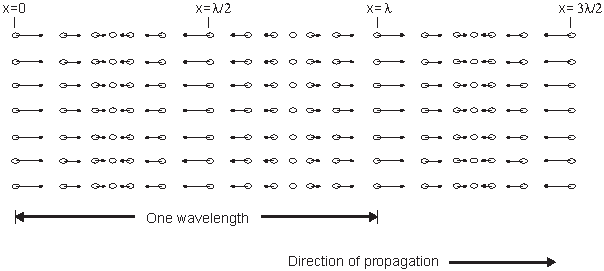
\includegraphics[width=.6\textwidth]{Figures/plane_wave_jensen-cropped.pdf}
	\caption{Particle displacement for a propagating ultrasound wave \cite{JensenUltrasoundBook}}
	\label{fig:planewave_jensen}
\end{figure}

\subsection{Comparison to Other Diagnostic Modalities}
Since medical imaging has been reportedly performed over 5 billion times as of 2004 \cite{Picano2004}, and later numbers from 2011 show a doubling of imaging per year, and a ten-fold increase in Ultrasound examinations between year 2000 and 2011 \cite{Szabo_UltrasoundBook_2}. Potentially millions of people have been spared painful exploratory surgery through noninvasive diagnostic imaging. Lives can be saved by diagnosis and timely intervention. Looking at \Cref{tab:imaging_modalities}, a comparison of each major diagnostic imaging method is seen. 
With x-rays, an important drawback is that patients are exposed to ionizing radiation when undergoing imaging. 
\cite{ShungUltrasound_Book,Shung1976,JensenUltrasoundBook,Jensen_Algorithms}
\cite{1999_SummerSchool_Notes,Szabo_UltrasoundBook_2}

\gls{dc} \gls{ltspice} \gls{matlab} \gls{mri} \gls{dsp}


\begin{table}[ht]
	\centering
	\begin{tabularx}{\textwidth}{@{}XXXXX@{}}
		\toprule
		\textbf{Modality} & \textbf{Ultrasound} & \textbf{X-ray} & \textbf{CT} & \textbf{MRI} \\ \midrule
		Topic              & Longitudinal, shear, mechanical properties              & Mean X-ray tissue absorbtion & Local tissue X-ray absorbtion & Biochemistry (\textit{T1} and \textit{T2})    \\
		Access             & Small windows adequate                                  & 2 sides needed               & Circumferential around body   & Circumferential around body \\
		Spatial resolution & Frequency and axially dependent, \SIrange{0.2}{3}{\milli\meter} & $\sim \SI{1}{\milli \meter}$           & $\sim \SI{1}{\milli \meter}$            & $\sim \SI{1}{\milli \meter}$          \\
		Penetration     & Frequency dependent, \SIrange{3}{25}{\centi\meter} & Excellent               & Excellent          & Excellent                                 \\
		Safety          & Excellent for > 50 years          & Ionizing radiation      & Ionizing radiation & Very good                                 \\
		Speed           & Real-time & Minutes & 20 minutes & Typical: 45 minutes, fastest: Real-time (\glsxtrshort{low-res}) \\
		Cost            & \$                                            & \$                      & \$\$                 & \$\$\$                                       \\
		Portability     & Excellent                                     & Good                    & Poor               & Poor                                      \\
		Volume coverage & Real-time 3D volumes, improving               & 2D                      & Large 3D volume    & Large 3D volume                           \\
		Contrast        & Increasing (shear)                            & Limited                 & Limited            & Slightly flexible                         \\
		Intervention    & Real-time 3D increasing                       & No, fluoroscopy limited & No                 & Yes, limited                              \\
		Functional      & Functional ultrasound                         & No                      & No                 & fMRI                                      \\ \bottomrule
	\end{tabularx}
	\caption{Comparison of Imaging Modalities \cite{Szabo_UltrasoundBook_2}}
	\label{tab:imaging_modalities}
\end{table}

%\begin{figure}[htbp]
%	\centering
%	\input{0_Figures/Introduction/ClassD_blockdiagram.tikz}
%	\caption{Block diagram of basic class-D amplifier topology.}
%	\label{fig:01_classd_diagram}
%\end{figure}

%See \autoref{fig:01_classd_diagram} for a block diagram overview of a class-D amplifier system with waveform illustrations.
%The primary benefit of the class-D topology is an increased power efficiency as the maximum theoretical power efficiency for class-D amplifiers are near 100\%, whereas Class-A- and Class-B amplifiers maximum theoretical power efficiency is 25\% and 78.5\%, respectively.\\
%
%The design process in this project will be based on previous work by \cite{multivar_ctrl_loops_for_SM_audio_systems,nagy_special_course}. These two works explored using LQR in a control loop and minimizing the generated noise within the circuit from that implementation. The result was a circuit design that was implemented in-house within the DTU laboratory that is documented through an iterative design process.

\section{Project scope}
As this project deals with a synthesis of a peculiar design and an analytical examination of a class-D system, this initial design will determine the specific direction of the qualitative analysis. The project is focused on the output stage of the system. Therefore analysis will comprise of distinctive variations of parasitic element combinations in the chosen output filter topology.

\subsection{Learning objectives}
See below for an outline of the project activities
\begin{table}[ht!]
	\centering
	\begin{tabular}{@{}l@{}}
		\toprule
		\textbf{Project specification}									\\ \midrule
		Learn a class-D amplifier topology, calculate component values	\\
		Understand and design a self-oscillating modulator amplifier	\\
		Investigate and test open loop output filter					\\
		Investigate and test closed loop output filter					\\
		Investigate output filter parasitic elements affects control loop\\
		Make quantifiable performance measurements on system			\\
		Write a technical report documenting the project work			\\ \bottomrule
	\end{tabular}
	\caption{Project specification table}
	\label{tab:specifications}
\end{table}

%\chapter{Introduction}
%The progress of imaging internal organs has advanced significantly during the \nth{20} century. Three major technologies used are X-ray, \gls{mri}, and ultrasound. Each of the technologies have distinct advantages and disadvantages in biomedical imaging, thus are still relevant for modern medicine. With x-rays, an important drawback is that patients are exposed to ionizing radiation 
%\cite{ShungUltrasound_Book,Shung1976,JensenUltrasoundBook,Jensen_Algorithms}
%\cite{1999_SummerSchool_Notes,Szabo_UltrasoundBook_2}
%This template complies with the DTU Design Guide \url{https://www.designguide.dtu.dk/}. DTU holds all rights to the design program including all copyrights. It is intended for two-sided printing. The \textbackslash \texttt{cleardoublepage} command can be used to ensure that new sections and the table of contents begins on a right-hand page. The back page always ends as an odd page. \cite{Jensen_Analysis_PW_1996}
%
%All document settings have been collected in Setup/Settings.tex. These are global settings, meaning the settings will affect the whole document. Defining the title for example will change the title on the front page, the copyright page, and the footer. A watermark can be enabled or disabled in Setup/Premeable.tex. You can edit the watermark to display draft, review, approve, confidential, or anything else. By default, the watermark is printed on top of the document's contents and has a transparent gray color. Here I am just testing the synchronization functionality of Overleaf and Github. Now, that the first synchronization finished successfully, I want to test that the reverse direction process is also functional. Hopefully, this will end up on Overleaf.
%
%\section{This is a section}
%Every chapter is numbered and the sections inherit the chapter number followed by a dot and a section number. Figures, equations, tables, etc. also inherit the chapter numbering. 
%
%\subsection{This is a sub section}
%Sub-sections are also numbered. In general, try not to use a deep hierarchy of sub-sections (\texttt{\textbackslash paragraph\{\}} and the like). The document will become segmented, which will make the document appear less coherent. 
%
%\subsubsection{This is a sub sub section}
%And those are not numbered. It is possible to adjust the deep hierarchy of numbering sections in Setup/Settings.tex. 
%
%The front and back cover has been made to replicate the examples in the design guide \url{https://www.designguide.dtu.dk/#stnd-printmedia}. The name of department heading is omitted because it is located in the top right corner (no need to write it twice). Take a look at \url{https://www.inside.dtu.dk/en/medarbejder/om-dtu-campus-og-bygninger/kommunikation-og-design/skabeloner/rapporter} if you want to make your cover separately. 
%
%Citing is done with the \texttt{biblatex} package \cite{1999_SummerSchool_Notes}. Cross referencing (figures, tables, etc.) is taken care by the \texttt{cleveref} package. Just insert the name of the label in \textbackslash \texttt{cref\{\}} and it will automatically format the cross-reference. For example, writing the \texttt{cleveref} command \textbackslash \texttt{cref\{fig:groupedcolumn\}} will output ``\cref{fig:groupedcolumn}''. Using \textbackslash \texttt{Cref\{\}} will capitalize the first letter and \textbackslash \texttt{crefrange\{\}\{\}} will make a reference range. An example: \Cref{fig:stackedbar} is an example of a stacked bar chart and \crefrange{fig:stackedcolumn}{fig:groupedcolumn} are three consecutive figures.
%
%\section{Font and symbols test}
%Symbols can be written directly in the document, meaning that there is no need for special commands to write special characters. I love to write special characters like æøå inside my \TeX{} document. Also á, à, ü, û, ë, ê, î, ï could be nice. So what about the ``¿'' character. What about ° é ® † ¥ ü | œ ‘ @ ö ä ¬ ‹ « © ƒ ß ª … ç ñ µ ‚ · ¡ “ £ ™ [ ] '. Some dashes - – —, and the latex form - -- --- 
%
%This is a font test \newline 
%Arial Regular \newline 
%%\textit{Arial Italic} \newline 
%%\textbf{Arial Bold} \newline 
%%\textbf{\textit{Arial Bold Italic}}
%
%\gls{mri}, \gls{snr}, \gls{smps}, \gls{rvs}, \gls{ac}, \gls{dc}, \gls{emi}, \gls{gcd}, \gls{lcm} \\
%\gls{high}, \gls{low}, \gls{spice}
%
%% Given a set of numbers, there are elementary methods to compute its \glsxtrlong{gcd}, which is abbreviated \glsxtrshort{gcd}. This process is similar to that used for \acrfull{lcm}.
%
%I want to talk about \gls{spice}, \gls{high} and \gls{low}. These are all \gls{dc} and \gls{ac} electric principles. I want to mention that \glsxtrlong{fet} devices can be called \glsxtrshort{fet}.
%
%\section{Tikz Test}
%\begin{figure}[h]
%	\centering 
%	\resizebox{\textwidth}{!}{
%		\begin{tikzpicture}
    [outer sep=0,
    >=latex,
    align=center]
    % Draw nodes
    \node[place]		(aud_in)	[draw=none]											{Audio\\input};
    \node[place]		(in_filt)	[inner sep=1mm,rectangle,right=4.5mm of aud_in]		{Input\\filter};
    \node[place]		(PI)		[inner sep=1mm,rectangle,right=4.5mm of in_filt]	{PI};
    \node[place]		(mod)		[inner sep=1mm,rectangle,right=4.5mm of PI]			{Modulator \&\\State feedback};
    \node[place]		(gate_drv)	[inner sep=1mm,rectangle,right=4.5mm of mod]		{Gate\\driver};
    \node[place]		(pwr_stg)	[inner sep=1mm,rectangle,right=4.5mm of gate_drv]	{Power\\stage};
    \node[place]		(LP_filt)	[inner sep=1mm,rectangle,right=4.5mm of pwr_stg]	{LPF};
    \node[place]		(spk)		[inner sep=1mm,rectangle,right=4.5mm of LP_filt]	{Speaker};
    \node[place]		(acq)		[inner sep=1mm,rectangle,below=4.5mm of mod]		{Acquisition\\circuits};
    % Draw lines between nodes
    \draw [|->] 		(aud_in) 		to 		(in_filt);
    \draw [->] 			(in_filt) 		to 		(PI);
    \draw [->]			(PI)			to		(mod);
    \draw [->]			(mod)			to		(gate_drv);
    \draw [->]			(gate_drv)		to		(pwr_stg);
    \draw [->]			(pwr_stg)		to		(LP_filt);
    \draw [->]			(LP_filt)		to		(spk);
    \draw [->]			(acq)			to		(mod);
    \draw [->]			(LP_filt)		|-		(acq);
    \draw [-]			(spk)			|-		(acq);
    \draw [->]			(acq)			-|		(PI);
\end{tikzpicture}
%	}
%	\caption{Simple overview of the system}
%	\label{fig:system_overview}
%\end{figure}
%
%I like to talk about logic systems and their binary states. Such as \gls{high} and \gls{low}. These are also important in \gls{spice} simulation systems.
%
%I like to explain abbreviations such as \glsxtrshort{fet}. This abbreviation stands for \glsxtrlong{fet}. I like this paper \cite{Omura2022}.
%Two datasheets \cite{AD8332,AD8333}. \gls{cad} \gls{dtu} \gls{kaist}. Signals are usually \glsxtrshort{ac}-coupled from the transducer.